\documentclass[11pt]{article}
\usepackage[scaled=0.92]{helvet}
\usepackage{geometry}
\geometry{letterpaper,tmargin=1in,bmargin=1in,lmargin=1in,rmargin=1in}
\usepackage[parfill]{parskip} % Activate to begin paragraphs with an empty line rather than an indent %\usepackage{graphicx}
\usepackage{amsmath,amssymb, mathrsfs,  mathtools, dsfont}
\usepackage{tabularx}
\usepackage{tikz-cd}
\usepackage[font=footnotesize,labelfont=bf]{caption}
\usepackage{graphicx}
\usepackage{xcolor}
%\usepackage[linkbordercolor ={1 1 1} ]{hyperref}
%\usepackage[sf]{titlesec}
\usepackage{natbib}
\usepackage{../../Tianpei_Report}

%\usepackage{appendix}
%\usepackage{algorithm}
%\usepackage{algorithmic}

%\renewcommand{\algorithmicrequire}{\textbf{Input:}}
%\renewcommand{\algorithmicensure}{\textbf{Output:}}



\begin{document}
\title{Lecture 4: Submersions, Immersions, and Embeddings}
\author{ Tianpei Xie}
\date{Oct. 17th., 2022}
\maketitle
\tableofcontents
\newpage
\section{Maps of Constant Rank}
\subsection{Submersions and  Immersions}
\begin{itemize}
\item The key linear-algebraic property of \emph{a linear map} is its \emph{\textbf{rank}}. In fact,  the rank is the \emph{\textbf{only property}} that distinguishes different linear maps if we are free to choose bases independently for the domain and codomain.

\item \begin{definition}
Suppose $M$ and $N$ are smooth manifolds with or without boundary. Given a smooth map $F: M \rightarrow N$ and a point $p \in M$, we define \underline{\emph{the \textbf{rank} of $F$ at $p$}} to be \emph{\textbf{the rank of the linear map} $dF_p: T_{p}M \rightarrow T_{F(p)}N$}; it is \underline{\emph{\textbf{the rank of the Jacobian matrix}}} of F in any smooth chart, or \emph{\textbf{the dimension of}} $\text{Im }dF_p \subseteq T_{F(p)}N$. If $F$ has the same rank $r$ \emph{at every point}, we say that it has constant rank, and write \underline{$\text{rank}\,F = r$}.
\end{definition}

\item \begin{definition}
Note that $\text{rank }dF_{p} \le \min\set{\text{dim }M, \; \text{dim }N}$. If the rank of $dF_p$ is equal to this upper bound, we say that \emph{\textbf{$F$ has full rank at $p$}}, and if $F$ has full rank everywhere, we say \underline{\emph{\textbf{$F$ has full rank}}}.
\end{definition}

\item \begin{definition}
The most important \emph{constant-rank maps} are those \emph{of full rank}. A smooth map $F: M \rightarrow N$ is called \underline{\emph{\textbf{a smooth submersion}}} if its differential is \underline{\emph{\textbf{surjective}}} \emph{at each point} (or \emph{\textbf{equivalently}}, if \underline{$\text{rank }F = \text{dim }N$}). 

It is called \underline{\emph{\textbf{a smooth immersion}}} if its differential is \underline{\emph{\textbf{injective}}} at each point (\emph{\textbf{equivalently}}, \underline{$\text{rank }F = \text{dim }M$}).
\end{definition}


\item \begin{remark} (\emph{\textbf{Submersion vs. Surjective and Immersion vs. Injective}})\\
A map $F: M \rightarrow N$ is \emph{surjective} if the preimage $F^{-1}(N)$ covers its domain $M$. It is submersion if \emph{\textbf{its differential}} $dF_p$ at $p$ is \emph{surjective} for all $p$. Similarly, $F$ is injective, if $F(a) \neq F(b)$ when $a \neq b$. It is immersion if \emph{\textbf{its differential}} $dF_p$ at $p$ is \emph{injective} for all $p$. 

The concept of \emph{\textbf{submersion/immersion}} is about \underline{\emph{\textbf{the local differential property}}} of $F$ while \emph{\textbf{the surjective/injective}} is about \underline{\emph{\textbf{the global property}}} of $F$.  Local property can be determined by the global property but not vice versa. Thus \emph{a map can be submersion but may not be surjective}.  \emph{A map can be immerison but may not be injective}. 
\end{remark}


\item \begin{proposition}
Suppose $F: M \rightarrow N$ is a smooth map and $p \in M$ . If $dF_p$ is \textbf{surjective}, then $p$ has a neighborhood $U$ such that $F|_{U}$ is a \textbf{submersion}. If $dF_p$ is \textbf{injective}, then $p$ has a neighborhood $U$ such that $F|_{U}$ is an \textbf{immersion}.
\end{proposition}

\item \begin{remark}
As we will see in this chapter, \emph{smooth submersions} and \emph{immersions} behave \emph{locally} like surjective and injective \emph{linear maps}, respectively. 
\end{remark}

\item \begin{example}(\emph{\textbf{Submersions and Immersions}}).
\begin{itemize}
\item Suppose $M_1,\ldots,M_k$ are smooth manifolds. Then each of \emph{\textbf{the projection maps}} $\pi_{i}: M_1\times \ldots \times M_k \rightarrow M_i$ is \emph{\textbf{a smooth submersion}}. In particular, \emph{the projection} $\pi: \bR^{n+k} \rightarrow \bR^n$ \emph{onto} the first $n$ coordinates is \emph{a smooth submersion}.
\item If $\gamma: J \rightarrow M$ is a smooth curve in a smooth manifold $M$ with or without boundary, then $\gamma$ is \emph{\textbf{a smooth immersion}} if and only if $\gamma'(t) \neq 0$ for all $t \in J$.
\item If $M$ is a smooth manifold and its tangent bundle $TM$ is given the smooth manifold structure described in Chapter 3, \underline{\emph{\textbf{the projection}}} $\pi: TM \rightarrow M$ is \emph{\textbf{a smooth submersion}}. 

To verify this, just note that with respect to any smooth local coordinates $(x^i)$ on an open subset $U \subseteq M$ and the corresponding natural coordinates $(x^i, v_i)$ on  $\pi^{-1}(U) \subseteq TM$, the coordinate representation of $\pi$ is $\widehat{\pi}(x, v) = x$.
\item The smooth map $X: \bR^2 \rightarrow \bR^3$ given by
\begin{align*}
X(u,v) =  ((2+ \cos(2\pi u))\cos(2\pi v),\, (2+\cos(2\pi u))\sin(2\pi v),\,\sin(2\pi u))
\end{align*} is a \emph{smooth immersion} of $\bR^2$ into $\bR^3$ whose image is the doughnut-shaped surface obtained by revolving the circle $(y -2)^2 + z^2 = 1$ in the $(y,z)$-plane about the $z$-axis .
\end{itemize}
\end{example}
\end{itemize}

\subsection{Local Diffeomorphisms}
\begin{itemize}
\item \begin{definition}
If $M$ and $N$ are smooth manifolds with or without boundary, a map $F: M \rightarrow N$ is called \underline{\emph{\textbf{a local diffeomorphism}}} if every point $p \in M$ has a neighborhood $U$ such that $F(U)$ is \emph{\textbf{open}} in $N$ and the restriction $F|_{U}: U \rightarrow F(U)$ is a \emph{\textbf{diffeomorphism}}. 
\end{definition}

\item The next theorem is the key to the most important properties of local diffeomorphisms.
\begin{theorem} (\textbf{Inverse Function Theorem for Manifolds}). \citep{lee2003introduction} \\
Suppose $M$ and $N$ are smooth manifolds, and $F: M \rightarrow N$ is a \textbf{smooth map}. If  $p \in M$ is a point such that $dF_p$ is \textbf{invertible}, then there are \textbf{connected} neighborhoods $U_0$ of $p$ and $V_0$ of $F(p)$ such that $F|_{U_0}: U_0 \rightarrow V_0$ is a \textbf{diffeomorphism}.
\end{theorem}

\item \begin{remark}
It is important to notice that we have stated Theorem above \emph{\textbf{only for manifolds without boundary}}. In fact, it can fail for a map whose domain has nonempty boundary.
\end{remark}

\item \begin{proposition} (\textbf{Elementary Properties of Local Diffeomorphisms}).
\begin{enumerate}
\item Every \textbf{composition} of local diffeomorphisms is a local diffeomorphism.
\item Every \textbf{finite product} of local diffeomorphisms between smooth manifolds is a local diffeomorphism.
\item Every local diffeomorphism is a \textbf{local homeomorphism} and \textbf{an open map}.
\item The \textbf{restriction} of a local diffeomorphism to an \textbf{open submanifold} with or without boundary is a local diffeomorphism.
\item Every \textbf{diffeomorphism} is a local diffeomorphism.
\item Every \textbf{bijective} local diffeomorphism is a diffeomorphism.
\item A map between smooth manifolds with or without boundary is a local diffeomorphism if and only if in a neighborhood of each point of its domain, it has a \textbf{coordinate representation} that is a \textbf{local diffeomorphism}.
\end{enumerate}
\end{proposition}

\item \begin{proposition}
Suppose $M$ and $N$ are smooth manifolds (without boundary), and $F: M \rightarrow N$ is \textbf{a map}.
\begin{enumerate}
\item $F$ is a local diffeomorphism if and only if it is \textbf{both} a \textbf{smooth immersion} and a \textbf{smooth submersion}.
\item If $\text{dim }M = \text{dim }N$ and $F$ is \textbf{either} a \textbf{smooth immersion} or a \textbf{smooth submersion}, then it is a local diffeomorphism.
\end{enumerate}
\end{proposition}
\end{itemize}

\subsection{The Rank Theorem}
\begin{itemize}
\item The most important fact about constant-rank maps is the following consequence of the inverse function theorem, which says that a constant-rank smooth map can be
placed locally into a particularly simple canonical form by a change of coordinates.

\item \begin{theorem} (\textbf{Rank Theorem}). \citep{lee2003introduction} \\
Suppose $M$ and $N$ are smooth manifolds of dimensions $m$ and $n$, respectively, and  $F: M \rightarrow N$ is a smooth map \underline{\textbf{with constant rank $r$}}. For each $p \in M$ there exist smooth charts $(U, \varphi)$ for $M$ centered at $p$ and $(V,\psi)$ for $N$ centered at $F(p)$ such that $F(U) \subseteq V$, in which $F$ has a \underline{\textbf{coordinate representation}} of the form
\begin{align}
\widehat{F}(x^1,\ldots, x^r, x^{r+1},\ldots, x^m) &= (x^1,\ldots, x^r, 0,\ldots, 0).  \label{eqn: rank_theorem_coordinate_rep}
\end{align} In particular, if $F$ is a \underline{\textbf{smooth submersion}}, this becomes
\begin{align}
\widehat{F}(x^1,\ldots, x^n, x^{n+1},\ldots, x^m) &=  (x^1,\ldots, x^n).  \label{eqn: rank_theorem_coordinate_rep_subm}
\end{align}
and if $F$ is a \underline{\textbf{smooth immersion}}, it is
\begin{align}
\widehat{F}(x^1,\ldots, x^m) &=  (x^1,\ldots, x^m, 0,\ldots, 0).  \label{eqn: rank_theorem_coordinate_rep_imm}
\end{align}
\end{theorem}

\item \begin{corollary}
Let $M$ and $N$ be smooth manifolds, let  $F: M \rightarrow N$ be a smooth map, and suppose $M$ is connected. Then the following are \textbf{equivalent}:
\begin{enumerate}
\item For each $p \in M$ there exist smooth charts containing $p$ and $F(p)$ in which \textbf{the coordinate representation of $F$ is linear}.
\item $F$ has \textbf{constant rank}.
\end{enumerate}
\end{corollary}

\item \begin{remark}
The canonical representation for a \emph{smooth submersion} in \eqref{eqn: rank_theorem_coordinate_rep_subm} is called the \emph{\textbf{canonical surjection}} or  \underline{\emph{\textbf{the projection map}}}, denoted as $\pi$;  Similarly, the canonical representation for a \emph{smooth immersion} in \eqref{eqn: rank_theorem_coordinate_rep_imm} is called the  \emph{\textbf{canonical injection}} or \underline{\emph{\textbf{the inclusion map}}}, denoted as $\iota$.

The Rank Theorem states that \underline{\emph{\textbf{every smooth immersion is an inclusion map locally}}} and \underline{\emph{\textbf{every smooth submersion is a projection map locally}}}, both regardless of the form of the map itself.
\end{remark}

\item The rank theorem is a purely \emph{\textbf{local statement}}. However, it has the following powerful \emph{\textbf{global} consequence}.
\begin{theorem} (\textbf{Global Rank Theorem}). \citep{lee2003introduction}\\
Let $M$ and $N$ be smooth manifolds, and suppose $F: M \rightarrow N$ is a smooth map of \textbf{constant rank}.
\begin{enumerate}
\item If $F$ is \textbf{surjective}, then it is a \textbf{smooth submersion}.
\item If $F$ is \textbf{injective}, then it is a \textbf{smooth immersion}.
\item If $F$ is \textbf{bijective}, then it is a \textbf{diffeomorphism}.
\end{enumerate}
\end{theorem}
\end{itemize}

\subsection{The Rank Theorem for Manifolds with Boundary}
\begin{itemize}
\item \begin{remark}
In the context of manifolds with boundary, we need the rank theorem only in one special case: that of a smooth immersion whose domain is a smooth manifold with
boundary. 
\end{remark}

\item \begin{theorem} (\textbf{Local Immersion Theorem for Manifolds with Boundary}). \citep{lee2003introduction} \\
Suppose $M$ is a smooth $m$-manifold with boundary, $N$ is a smooth $n$-manifold, and $F: M \rightarrow N$ is a smooth immersion. For any $p \in \partial M$; there exist a smooth boundary chart $(U,\varphi)$ for $M$ centered at $p$ and a smooth coordinate chart $(V, \psi)$ for $N$ centered at $F(p)$ with $F(U) \subseteq V$, in which $F$ has the coordinate representation
\begin{align}
\widehat{F}(x^1,\ldots, x^m) &=  (x^1,\ldots, x^m, 0,\ldots, 0) \label{eqn: local_immersion}
\end{align}
\end{theorem}
\end{itemize}

\section{Embeddings}
\subsection{Definitions}
\begin{itemize}
\item  One special kind of \emph{\textbf{immersion}} is particularly important.
\begin{definition}
If $M$ and $N$ are smooth manifolds with or without boundary, a  \underline{\emph{\textbf{smooth embedding}}} of $M$ into $N$ is a \underline{\emph{\textbf{smooth immersion}}} $F: M \rightarrow N$ that is \emph{\textbf{also}} \underline{\emph{\textbf{a topological embedding}}}, i.e., \emph{a \textbf{homeomorphism} onto its image} $F(M) \subseteq N$ in the \emph{subspace topology}. 
\end{definition}

\item \begin{remark}
\emph{\textbf{A smooth embedding}} is a map that is \emph{\textbf{both}} a \emph{\textbf{topological embedding}} and a \emph{\textbf{smooth immersion}}, not just a topological embedding that happens to be smooth. 

Also a map is a \textbf{\emph{smooth embedding}} $\Rightarrow$ \emph{\textbf{the map is an injective smooth immersion}}. The reverse is \textbf{not} necessarily \textbf{true} since this map also need to have \emph{\textbf{continuous inverse}} from $F(M)$ to domain $M$.
\end{remark}

\item \begin{example}(\emph{\textbf{Smooth Embeddings}}).
\begin{enumerate}
\item  If $M$ is a smooth manifold with or without boundary and $U \subseteq M$ is an \emph{\textbf{open submanifold}}, the \emph{\textbf{inclusion map}} $U \xhookrightarrow{} M$ is a smooth embedding.
\item If $M_1,\ldots,M_k$ are smooth manifolds and $p_i \in M_i$ are arbitrarily chosen points, each of the maps $\iota_{j}: M_j \rightarrow M_1\times \ldots \times M_k$ given by
\begin{align*}
\iota_{j}(q) &= \paren{p_1, \ldots, p_{j-1}, q, p_{j+1}, \ldots, p_{k}}
\end{align*} is \emph{\textbf{a smooth embedding}}. In particular, the inclusion map $\bR^n \xhookrightarrow{} \bR^{n+k}$ given by sending $(x^1,\ldots,x^n)$ to $(x^1,\ldots,x^n, 0,\ldots, 0)$  is \emph{a smooth embedding}.
\item The smooth map $X: \bR^2 \rightarrow \bR^3$ given by
\begin{align*}
X(u,v) =  ((2+ \cos(2\pi u))\cos(2\pi v),\, (2+\cos(2\pi u))\sin(2\pi v),\,\sin(2\pi u))
\end{align*} descends to \emph{\textbf{a smooth embedding}} of the \emph{\textbf{torus}} $\bS^1\times \bS^1$ into $\bR^3$.
\end{enumerate}
\end{example}

\item \begin{remark}
To understand more fully what it means for a map to be a smooth embedding, it is useful to bear in mind some examples of \emph{\textbf{injective} smooth maps that are \textbf{not smooth embeddings}}. 
\begin{enumerate}
\item \begin{example}
The map $\gamma: \bR \rightarrow \bR^2$ given by $\gamma(t) = (t^3, 0)$ is a smooth map and \emph{\textbf{a topological embedding}}, but it is \emph{\textbf{not a smooth embedding}} because $\gamma'(0) = 0$. (i.e. it is \emph{\textbf{not a smooth immerision}}.)
\end{example}

\item \begin{example} (\emph{\textbf{A Dense Curve on the Torus}}). Let $\mathbb{T}^2  = \bS^1 \times \bS^1 \subseteq \bC^2$ denote the torus, and let $\alpha$ be any \emph{\textbf{irrational number}}. The map $\gamma: \bR \rightarrow \mathbb{T}^2$ given by
\begin{align*}
\gamma(t) &= \paren{e^{2\pi i t}, e^{2\pi i \alpha t}} 
\end{align*} is a \emph{smooth immersion} because $\gamma'(t)$ never vanishes. It is also \emph{injective}, because $\gamma(t_1) = \gamma(t_2)$ implies that both $t_1 - t_2$ and  $\alpha t_1 - \alpha t_2$ are integers, which is impossible unless $t_1 = t_2$.

Consider the set $\gamma(\mathbb{Z}) = \set{\gamma(n): n \in \mathbb{Z}}$. It follows from Dirichlet’s approximation theorem that $\gamma(0)$ is a limit point of $\gamma(\mathbb{Z})$. But this means that $\gamma$ is \emph{\textbf{not a homeomorphism}} onto its image, because $\mathbb{Z}$ has no limit point in $\bR$. 
\end{example}

\item \begin{example} (\emph{\textbf{The Figure-Eight Curve}}). \\ 
Consider the curve  $\beta: (-\pi, \pi) \rightarrow \bR^2$ defined by
\begin{align*}
\beta(t) &= (\sin 2t,  \sin t).
\end{align*} Its image is a set that looks like a figure-eight in the plane, sometimes called a \emph{\textbf{lemniscate}}. (It is the locus of points $(x,y)$ where $x^2 =4y^2(1-y^2)$, as you can check.) It is easy to see that $\beta$ is an \emph{\textbf{injective smooth immersion}} because $\beta'(t)$ never vanishes; but it is \emph{\textbf{not a topological embedding}}, because its image is compact in the subspace topology, while its domain is not.
\end{example}
\end{enumerate}
\end{remark}


\item \begin{proposition}
Suppose $M$ and $N$ are smooth manifolds with or without boundary, and $F: M \rightarrow N$ is an \textbf{injective smooth immersion}. If \textbf{any} of the following holds, then $F$ is a\textbf{ smooth embedding}.
\begin{enumerate}
\item $F$ is an \textbf{open} or \textbf{closed} map. (i.e. it maps an open/closed set to an open/closed set)
\item $F$ is a \textbf{proper map}. (i.e. the preimage of every compact set is compact)
\item $M$ is \textbf{compact}.
\item $M$ has empty boundary and $\text{dim }M = \text{dim }N$
\end{enumerate}
\end{proposition}

\item \begin{theorem} (\textbf{Local Embedding Theorem}).  \citep{lee2003introduction}\\
Suppose $M$ and $N$ are smooth manifolds with or without boundary, and $F: M \rightarrow N$ is a smooth map. Then $F$ is a \textbf{smooth immersion} if and only if every point in $M$ has a neighborhood $U\subseteq M$ such that $F|_{U}: U \rightarrow N$ is a \textbf{smooth embedding}.
\end{theorem}

\item \begin{definition}
If $X$ and $Y$ are topological spaces, a continuous map $F: M \rightarrow N$ is called \emph{\textbf{a topological immersion}} if every point of $X$ has a neighborhood $U$ such that $F|_{U}$ is a \textbf{topological embedding}. 
\end{definition}

\item \begin{remark}
Thus, \textbf{every smooth immersion is a topological immersion}; but, just as with embeddings, a topological immersion that happens to be smooth need not be a smooth immersion.
\end{remark}
\end{itemize}

\section{Submersions}
\begin{itemize}
\item \begin{definition}
If $\pi: M \rightarrow N$ is any continuous map, a \underline{\emph{\textbf{section}}} of $\pi$ is a \underline{\emph{\textbf{continuous right inverse}}} for $\pi$, i.e., a continuous map $\sigma: N \rightarrow M$ such that $\pi \circ \sigma = \text{Id}_N$:
\[
  \begin{tikzcd}
     M  \arrow{r}{\pi}  & N   \arrow[l, bend left,  "\sigma"] 
  \end{tikzcd}
\] 
\end{definition}

\item \begin{definition}
A \emph{\textbf{local section}} of $\pi$ is a continuous map $\sigma: U \rightarrow M$ defined on some open subset $U \subseteq N$ and satisfying the analogous relation $\pi \circ \sigma = \text{Id}_U$
\end{definition}


\begin{figure}
\begin{minipage}[t]{1\linewidth}
  \centering
  \centerline{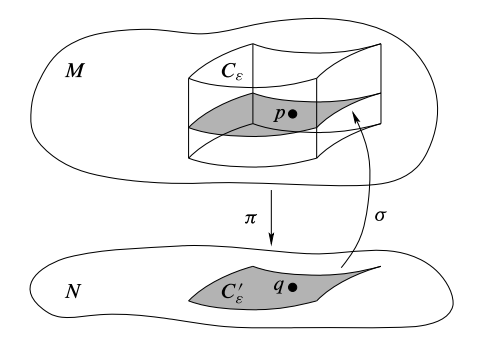
\includegraphics[scale = 0.4]{local_section_of_submersion.png}}
\end{minipage}
\caption{\footnotesize{\textbf{The local section of a submersion. \citep{lee2003introduction}}}}
\label{fig: local_section_of_submersion}
\end{figure}



\item \begin{theorem} (\textbf{Local Section Theorem}). \citep{lee2003introduction}\\
Suppose $M$ and $N$ are smooth manifolds and $\pi: M \rightarrow N$ is a smooth map. Then $\pi$ is a \textbf{smooth submersion} if and only if \textbf{every point} of $M$ is in the \textbf{image} of a \textbf{smooth local section} of $\pi$.
\end{theorem}

\item \begin{definition}
If $X$ and $Y$ are topological spaces, a continuous map $\pi: M \rightarrow N$ is called \emph{\textbf{a topological submersion}} if every point of $X$ is in the \textbf{image} of a \textbf{(continuous) local section} of $\pi$. 
\end{definition}

\item \begin{proposition} (\textbf{Properties of Smooth Submersions}). \\
Let $M$ and $N$ be smooth manifolds, and suppose $\pi: M \rightarrow N$ is a smooth submersion. Then $\pi$ is \textbf{an open map}, and if it is \textbf{surjective} it is a \textbf{quotient map}.
\end{proposition}

\item The next three theorems provide important tools that we will use frequently
when studying submersions. 
\begin{theorem} (\textbf{Characteristic Property of Surjective Smooth Submersions}).\\
Suppose $M$ and $N$ are smooth manifolds, and $\pi: M \rightarrow N$ is a \textbf{surjective smooth submersion}. For any smooth manifold $P$ with or without boundary, a map $F: N \rightarrow P$ is \textbf{smooth} if and only if $F \circ \pi$ is \textbf{smooth}:
\[
  \begin{tikzcd}
     M  \arrow[swap]{d}{\pi} \arrow[dr, "F \circ \pi"]  & \\
     N   \arrow[r, swap,  "F"]  & P.
  \end{tikzcd}
\] 
\end{theorem}


\begin{theorem} (\textbf{Passing Smoothly to the Quotient}).\\
Suppose $M$ and $N$ are smooth manifolds and  $\pi: M \rightarrow N$  is a \textbf{surjective smooth submersion}. If $P$ is a
smooth manifold with or without boundary and $F: M \rightarrow P$ is a smooth map that is \textbf{constant} on \textbf{the fibers of $\pi$}, then there exists a \textbf{unique smooth map} $\widetilde{F}: N \rightarrow P$ such that $\widetilde{F} \circ \pi = F$:
\[
  \begin{tikzcd}
     M  \arrow[swap]{d}{\pi} \arrow[dr, "F"]  & \\
     N   \arrow[r, swap, dashed,  "\widetilde{F}"]  & P.
  \end{tikzcd}
\] 
\end{theorem}

\begin{theorem} (\textbf{Uniqueness of Smooth Quotients}). \\
Suppose that $M, N_1$, and $N_2$ are smooth manifolds, and $\pi_1: M \rightarrow N_1$ and $\pi_2: M \rightarrow N_2$ are \textbf{surjective smooth submersions} that are \textbf{constant} on \textbf{each other's fibers}. Then there exists a \textbf{unique diffeomorphism} $F: N_1 \rightarrow N_2$ such that $F\circ \pi_1 = \pi_2$:
\[
  \begin{tikzcd}
     & M  \arrow[swap]{dl}{\pi_1} \arrow[dr, "\pi_2"]  & \\
     N_1   \arrow[rr, swap, dashed,  "F"]  & & N_2.
  \end{tikzcd}
\] 
\end{theorem}

\end{itemize}

%\section{Smooth Covering Maps}


\newpage
\bibliographystyle{plainnat}
\bibliography{book_reference.bib}
\end{document}